\section{Seleção de modelo}
Para realização desta etapa, foi desenvolvido um algoritmo que divide o conjunto total de exemplos de treino, em um conjunto de treino, um de validação e outro de testes. Nota-se que os elementos para todos os conjuntos são escolhidos de maneira aleatória pois caso contrário poderíamos poderíamos ter um conjunto enviesado e também que os testes foram realizados sobre a arquitetura com uma camada escondida que possui vinte e cinco neurônios (arquitetura original), pois o aumento de camadas e de neurônios não resultou em um aumento significativo de acurácia.
\begin{figure}[htb]
    \centering
    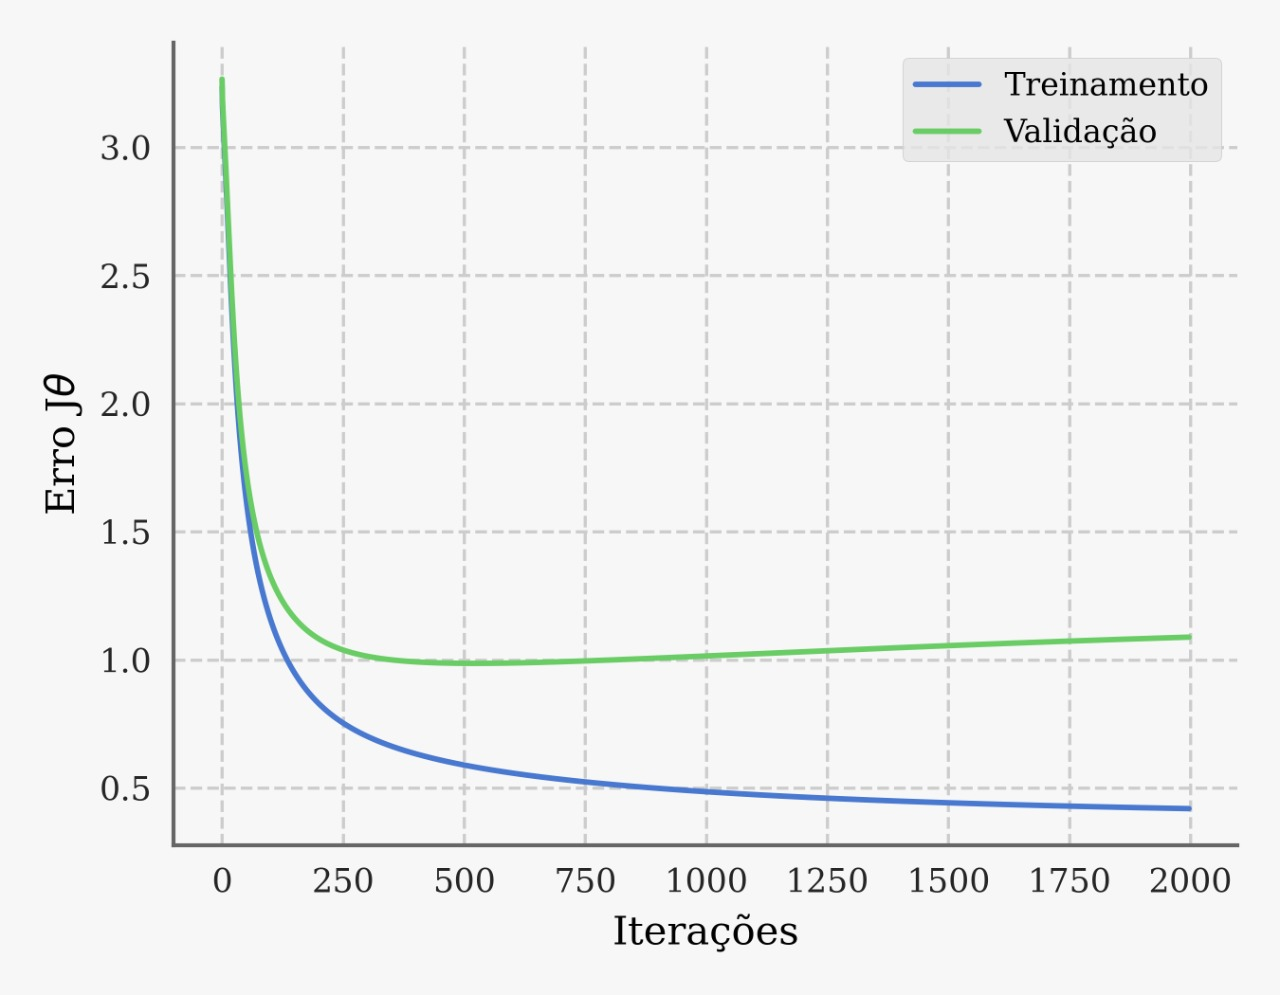
\includegraphics[width=0.8\linewidth]{graficos/erro_lambda1.png}
    \caption{Função de erro calculada para $\lambda $ igual a 1.}
    \label{fig:custo1}
\end{figure}
\subsection{Seleção dos lambdas}
Para se obter o melhor valor de lambda, realizamos o cálculo do erro para uma quantidade fixa de iterações, desta forma escolhemos o lambda ideal como aquele que mais reduz a função de custo.
\begin{figure}[htb]
    \centering
    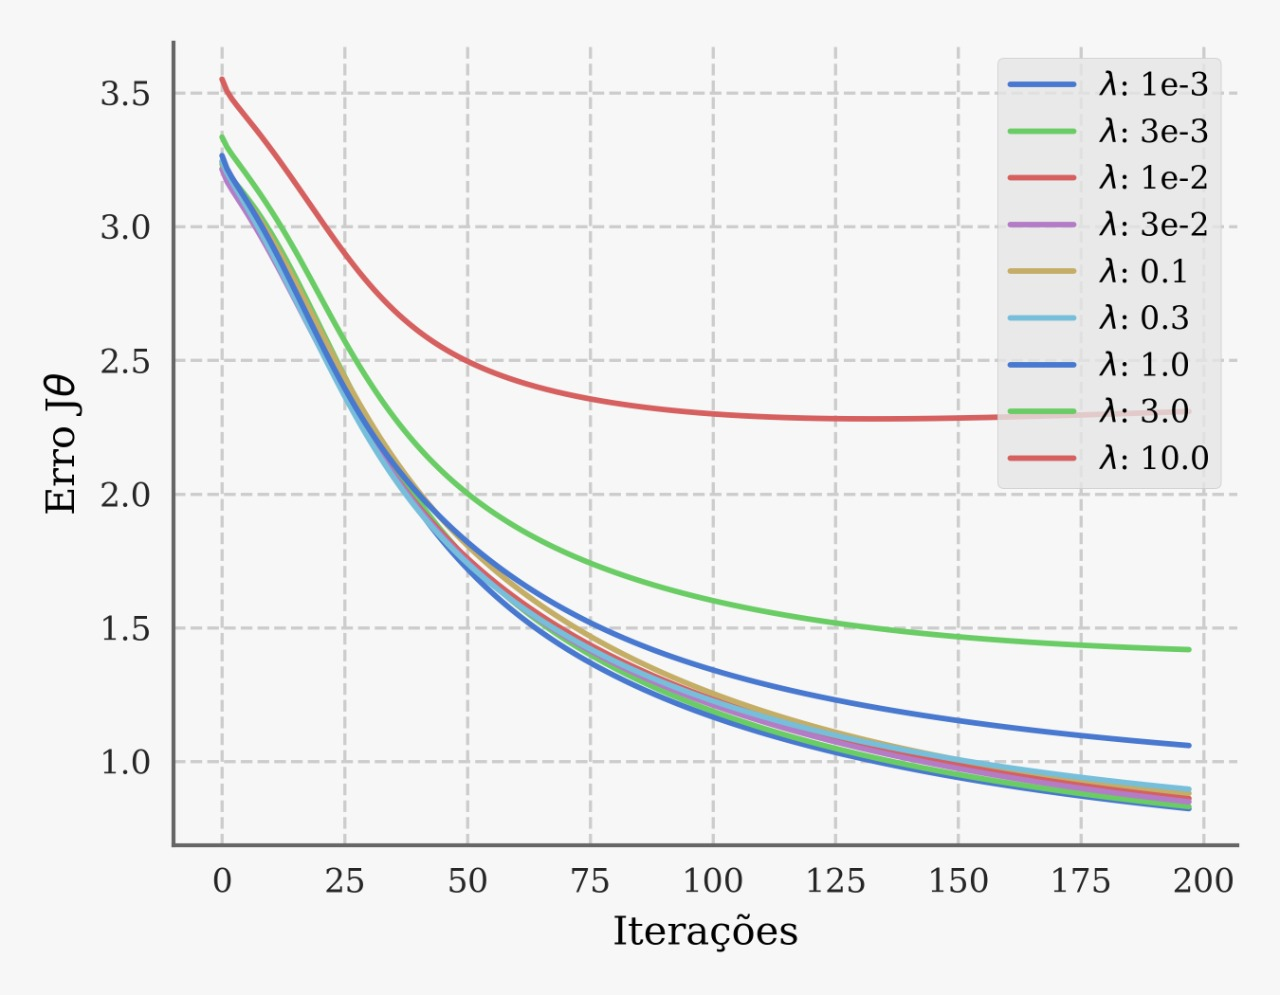
\includegraphics[width=0.60\linewidth]{graficos/teste_lambda.png}
    \caption{Testes realizados para escolha de $\lambda$.}
    \label{fig:lambda}
\end{figure}

Nota-se que que o valor com maior eficiência, ou seja, aquele que mais reduziu o custo foi $ \lambda $ igual a 0.001 como mostra a figura \ref{fig:zoom}
\begin{figure}[htb]
    \centering
    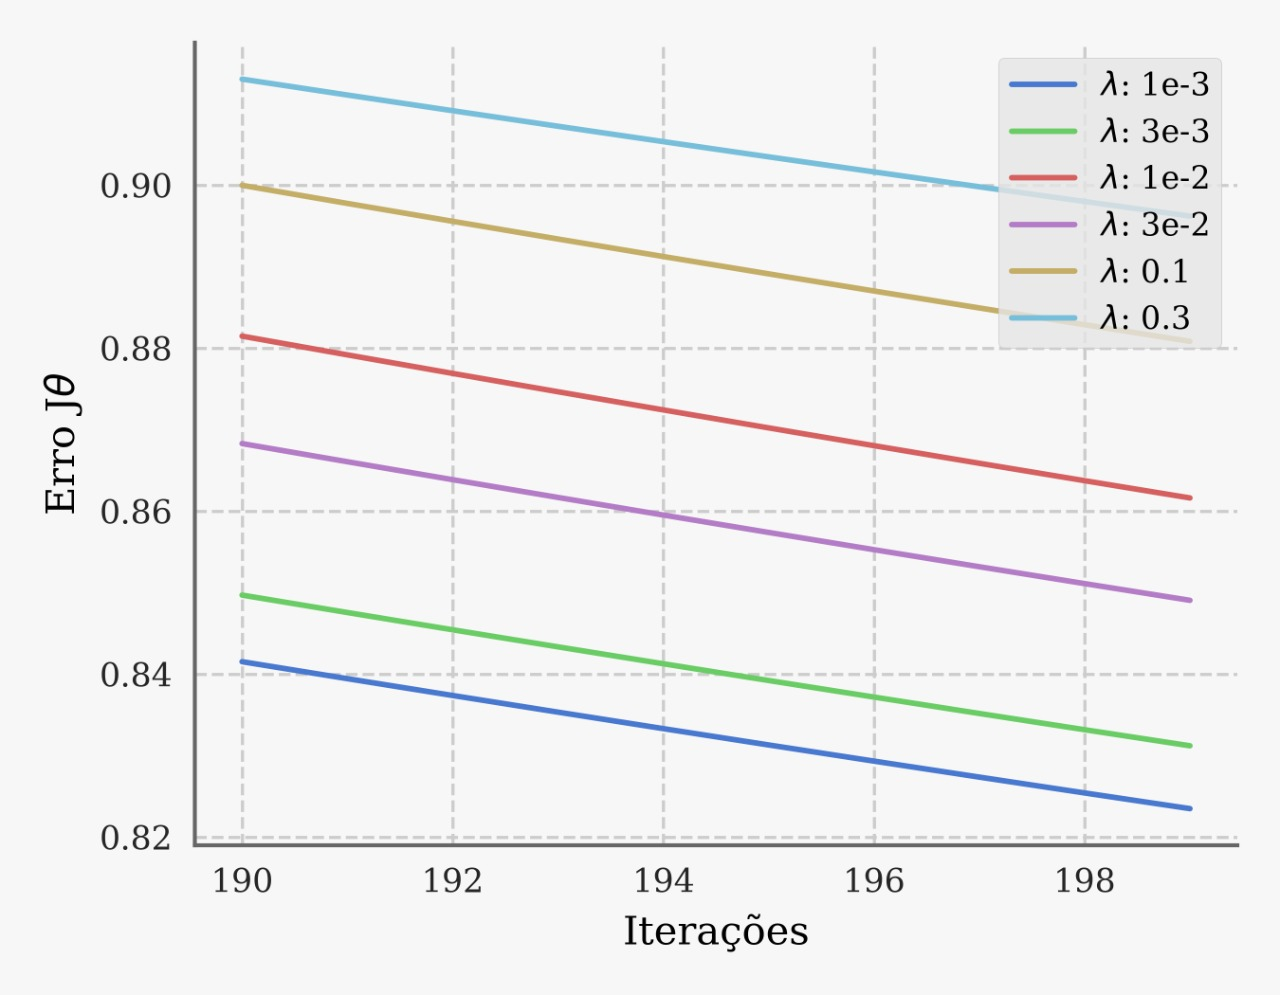
\includegraphics[width=0.64\linewidth]{graficos/zoom.png}
    \caption{Testes realizados para escolha de $\lambda$.}
    \label{fig:zoom}
\end{figure}
\newpage
Portanto, ao calcularmos novamente o grafico que representa o erro de validação, mas desta vez com o lambda otimizado temos o seguinte gráfico:
\begin{figure}[htb]
    \centering
    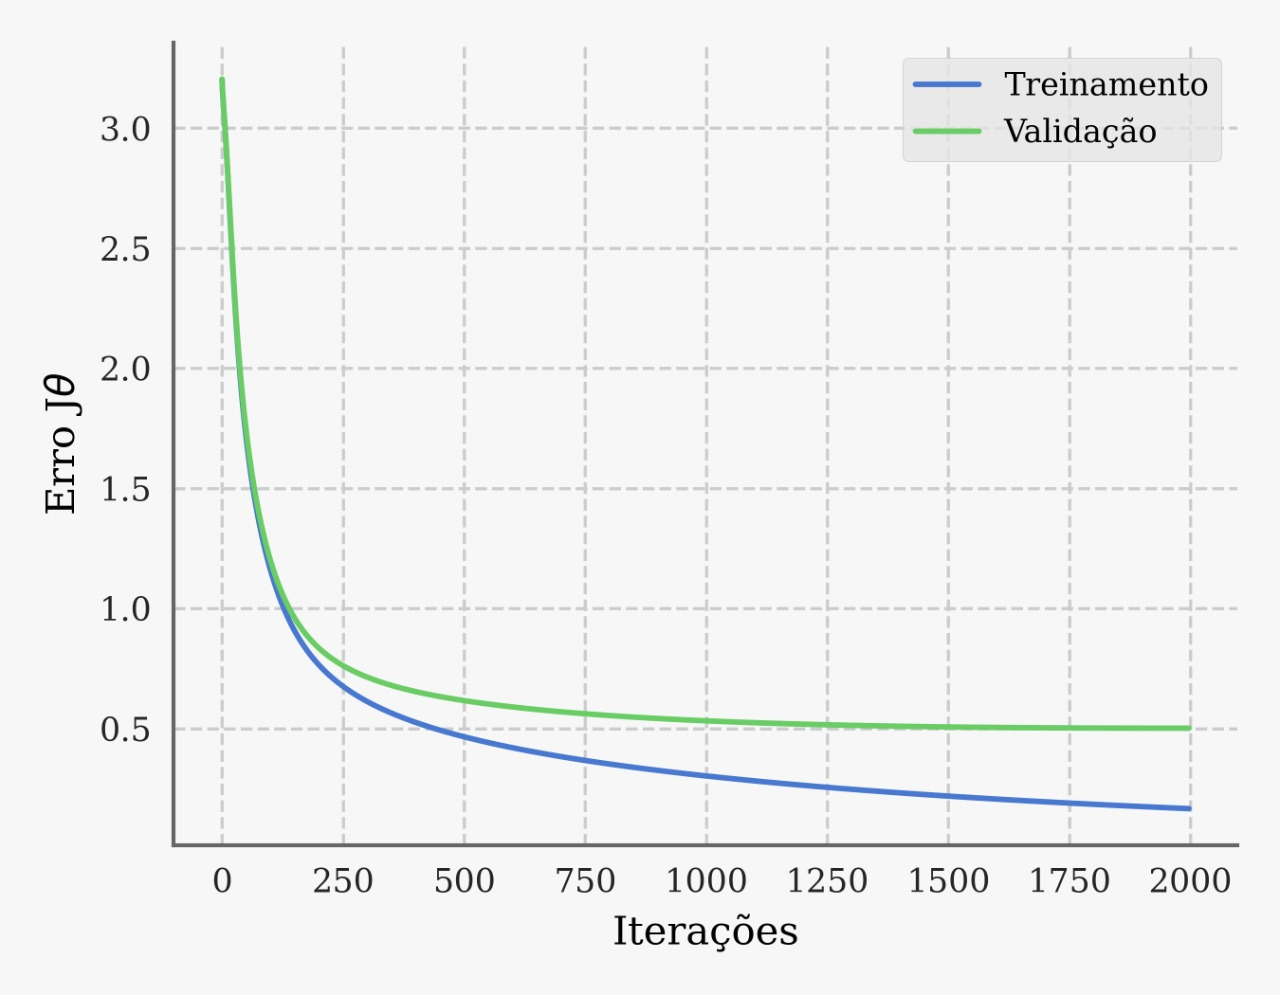
\includegraphics[width=0.8\linewidth]{graficos/erro_lambda_great.png}
    \caption{Testes realizados com $\lambda $ otimizado.}
    \label{fig:otimizado}
\end{figure}

É visível pela figura \ref{fig:otimizado} que a partir de uma certa 
quantidade de iterações a função de custo para o conjunto de validação 
atinge uma assíntota $h(x)$ igual a uma constante (neste caso 0.5) portanto mesmo que o treinamento 
siga diminuindo lentamente a validação não segue a mesma tendência.

Por fim, obtemos uma acurácia no conjunto de testes igual a 92.30\% utilizando de uma arquitetura com uma camada escondida que possui 25 neurônios, com taxa de aprendizado $\alpha$ igual a 1  e $\lambda$ igual a 0.001.

